\chapter{Automated debugging techniques}

\change[inline]{TODO: Link relevant literature from Slicing of LLVM bitcode (muni.cz) and Bobox Runtime Optimization (cuni.cz)}

Debugging can be described as the process of analyzing erroneous code to find 
the cause of those errors. 
Errors can also be of different natures.
It can for example stem from poor design of the application.
If that is not the case, then perhaps it comes from a rarely
encountered input or a corner-case. 
The flaw might also be present
in external code such as libraries or inappropriate usage of
existing technologies.

It can be said with confidence that debugging is rarely an algorithmic
approach.
While the goal is clear, the process of debugging depends entirely 
on the programmer.
It is typical that developers try to look for a root cause
of an error by feeling what might be wrong.
This works rather well in code the programmer is familiar with.
However, in larger projects the developer did not create by himself,
more sophisticated and reliable approaches are required.
For example, one might add logging to the code being debugged,
or perhaps create more tests that can narrow down the errorneous code.

All of the mentioned techniques require either the knowledge of the code 
or enough time to write supporting code. Additional time might be spent
looking through the logs and executing tests. Therefore, it is rather
hard to tell beforehand how much time and resources debugging will take.

While most developers see debugging as a manual chore, there were numerous 
attempts~at automating at least some parts of it during the last few decades. 
The rise in popularity of program analysis resulted in automated error checks 
for popular programming languages. 

Although these checks mostly cover only specific 
cases~of potential bugs, such as out-of-range array indexing, they have proven 
themselves as a useful tool for the developer. In the context of this work, 
such checks provide a helping hand at a low cost when minimizing a program. 

The following sections will talk about the techniques behind such checkers 
and how they deal with automated debugging. Notably, they describe
the motivation and notation of Delta debugging and static and dynamic
slicing.

\section{Delta debugging}

Delta debugging is an iterative approach described by \citet{Zeller99}.
\change{TODO: Link the reference number in brackets, i.e. Zeller [X]}
It does not perform any static analysis of the debugged program, as it 
is~not meant to find failures in the code. 

Delta debugging instead intends to 
minimize the debugged program's incorrect input to isolate the input's 
failure-inducing part. 
Therefore, it requires the program in question and the specific input 
and the expected output. 
In other words, Delta debugging requires a set of test cases, which attempts to 
minimize and isolate the failure-inducing input. 
In order to understand where
this app\-roach came from, we need to define several important properties of 
programs and test cases presented by \citet{Zeller02}.
\change{TODO: Link the reference number in brackets, i.e. Zeller [X]}

\begin{defn}[Test case]\label{def02:1}
  Let $c_\mathcal{F}$ be a set of all changes $\delta_1,\dots,\delta_n$ 
  between a passing program run $r_\mathcal{P}$ and a failing program run
  $r_\mathcal{F}$ such that 
  \begin{align}
	r_\mathcal{F} = (\delta_1(\delta_2(\dots(\delta_n(r_\mathcal{P}))))). \nonumber 
  \end{align}
  We call a subset $c \subseteq c_\mathcal{F}$ a \emph{test case}.
\end{defn}

Test runs should differ based on program's code. 
The definition states that making changes to the program,
i.e. applying a function that alters the code, enough times
and well enough to transform a passing program to a failing one,
results in a test case.

\begin{defn}[Global minimum]\label{def02:2}
  A test case $c \subset c_\mathcal{F}$ is called a \emph{global minimum}
  of $c_\mathcal{F}$ if $\forall c_i \subseteq c_\mathcal{F}:
  (|c_i| < |c| \implies c_i$ does not cause the program to fail.$)$
\end{defn}

Global minimum can be interpreted as the smallest set of changes able to
make the program fail.

\begin{defn}[Local minimum]\label{def02:3}
  A test case $c \subset c_\mathcal{F}$ is called a \emph{local minimum}
  of $c_\mathcal{F}$ if $\forall c_i \subseteq c:
  (c_i$ does not cause the program to fail.$)$
\end{defn}

The aforementioned minimality is defined as follows.

\begin{defn}[$n$-minimality]\label{def02:4}
  A test case $c \subset c_\mathcal{F}$ is \emph{$n$-minimal}
  if $\forall c_i \subseteq c:
  (|c| - |c_i| \leq n \implies c_i$ does not cause the program to fail.$)$
\end{defn}

The minimizing Delta debugging algorithm attempts to find a 1-minimal test case.

Delta debugging seems to bet on the premise that large-scale applications are written
with automated testing in mind. On the same note, it is the recommended practice to
develop programs while at the same time dedicating resources to write tests for that
program.

The defined minimality can be used to construct the minimizing algorithm. 
However, the delta debugging algorithm can be easily and more comprehensively explained 
without the definition as well.

\change[inline]{TODO: Move comments more towards the center.}

\begin{algorithm}
	\label{alg:dd}
	\caption{Minimizing Delta Debugging Algorithm} 
	\begin{algorithmic}[1]
		\State $n \leftarrow 2$
		\State Split a string $\sigma$ into $\alpha_1,\dots,\alpha_n$ of equal size.
		\Comment Where $\sigma$ is test's input.
		\State For each $\alpha_i$, calculate its complement $\beta_i$.
		\State Run tests on $\alpha_1,\dots,\alpha_n,\beta_1,\dots,\beta_n$.
		\If{all tests passed}
			\State $n \leftarrow 2*n$
			\If{$n > |\sigma|$}
				\Return the most recent failure causing substring.
			\Else
				\State goto (2).
			\EndIf
		\ElsIf{$\alpha_i failed$}
			\State $n \leftarrow 2$.
			\State $\sigma \leftarrow \alpha_i$.
			\If{$|\sigma| == 1$}
				\Return $\sigma$.
			\Else
				\State goto (2).
			\EndIf
		\Else
			\Comment $\beta_i$ failed.
			\State $\sigma \leftarrow \beta_i$.
			\State $n \leftarrow n - 1$.
			\State goto (2).
		\EndIf
	\end{algorithmic} 
\end{algorithm}

The simplified algorithm seen in~\ref{alg:dd} splits the input into $n$ even-sized
parts and their respective complements. 
Tests are then applied to these snippets, which can result in three different outcomes. 
If all tests pass correctly, the granularity, i.e., $n$, is doubled, and the input is split
into more even-sized parts. 
On the other hand, if a snippet fails a test, the granularity is reset to its initial value.
Furthermore, the snippet now becomes the input. 
If neither of the two mentioned scenarios happens, 
then a snippet's complement must have failed to pass a test. 
This case results in the granularity being decreased, 
and the input is set to the failure causing complement.
These three actions repeat iteratively, updating the input and 
splitting it systematically with different granularities. 
Once the granularity is greater than the input's size, 
the most recent failure-inducing snippet is returned. 
The same case holds when the input is of size $1$, i.e., it cannot be further divided.

Additionally, minimizing is not the only approach Delta debugging suggests.
A more sophisticated one is isolation. Minimization can be described as removing parts
while the failure persists, which means that the output changes are only made in failing
iterations.
Isolation extends this by adding failure-inducing differences while the program passes tests.
This addition results in changes in both the passing and failing iterations.

One can quickly transform the input minimalization of Delta debugging into either source
code minimalization or error isolation at both the compile-time and runtime.
This transformation can be achieved for the compile-time by first setting the input
as the debugged program's source code. 
Second, it is required to set the expected
output to either 'compiled' or 'failed to compile'. 
Finally, the input is fed into a compiler, for example, GCC, which produces
one of the two set outputs. 

The runtime variant only differs in two points—first, changing the expected outputs. 
Second, changing the compiler to a compiler-debugger pipeline so that the source 
can be compiled and run.

\section{Static slicing}

Program slicing, formalized more than three decades ago,
is a branch of program analysis that studies program semantics.
It systematically observes and alters the program's control-flow
and data-flow for a given statement and variable in the code.  
The goal of slicing is to create a slice of a program,
i.e., a series of parts of the program that could potentially
impact the control and data flow at some given point in that program. 
The direction from which the target statement is approached divides 
slicing methods into two groups. 
Firstly, forward slicing uncovers parts of the code that 
might be affected by the targeted statement and variable. 
Secondly, and much more common, backward slicing computes 
parts of the program that impacts the targeted statement.

The first introduced slicing method was static backward slicing.
And with it came brand new formalism concerning program analysis. 
Specifically for static slicing methods, definitions for the target 4
statement and variable needed to be written.
\citet{Weiser84}\change{TODO: Link the reference number in brackets, i.e. Zeller [X]}
defined a slice with respect to criterion C 
as a part of a program that potentially affects given variables in a given point. 

\begin{defn}[Static slicing criterion]\label{def02:5}
  Let $\mathcal{P}$ be a program consisting of program points 
  $P = p_1,\dots,p_n$ and variables $V = v_1,\dots,v_m$.
  Any pair $C = (p_i, V')$, such that $p_i \in P$, $V' \subseteq V$, and 
  $\forall v_i \in V': v_i$ is present in $p_i$, 
  is called a \emph{slicing criterion}.
\end{defn}

Slicing is the process of finding such a part of a program. 
Suggested approaches neglected any execution information and 
focused solely on observations made by analyzing the code.

\begin{minipage}{0.46\textwidth}
\begin{lstlisting}[basicstyle=\tiny, caption=Simple branching pro\-gram,
  language=C++, label={lst:simpleexample}]
#include<iostream>

void write(int x)
{
	std::cout << x << "\n";
}

int read()
{
	int x;
	std::cin >> x;
	
	return x;
}

int main(void)
{
	int x = 1;
	int a = read();
	
	for (int i = 0; i < 0xffff; i++)
	{
		write(i);
	}
	
	if ((a % 2) == 0)
	{
		if (a != 0)
		{
			x *= -1;
		}
		else
		{
			x = 0;
		}
	}
	else
	{
		x++;
	}

	write(x);

	return 0;
}
\end{lstlisting}
\end{minipage}
\hfill
\begin{minipage}{.45\textwidth}
\begin{lstlisting}[basicstyle=\tiny, caption=Static slice of the simple 
  branching program, language=C++, numbers=right,
  label={lst:staticslice}]
#include<iostream>

void write(int x)
{
	std::cout << x << "\n";
}

int read()
{
	int x;
	std::cin >> x;
	
	return x;
}

int main(void)
{
	int x = 1;
	int a = read();
		
	
	
	

	
	if ((a % 2) == 0)
	{
		if (a != 0)
		{
			x *= -1;
		}
		else
		{
			x = 0;
		}
	}
	else
	{
		x++;
	}

	write(x);

	return 0;
}
\end{lstlisting}
\end{minipage}

One can imagine that the size of a static slice would be much smaller
than the original program. 
That would be the case in modular code that rarely interacts between
its components. 
An example of such code would be heavy parallel applications and 
computational tasks. 
However, in programs with aggressive use of branching, it is not so. 
Since static slicing considers statements that \textbf{might} 
impact the criterion, it leaves otherwise useless branches in the slice,
thus negating the potential decrease in size. 

In listing~\ref{lst:simpleexample}, we can see the code of a simple program.
It loads a value $a$, which then alters the control-flow of the code.
Meanwhile, it iterates through a printing loop. 
The intriguing part, however, is the output of the $write(x)$ 
command on line $42$. 
Let the criterion be $C = (write(x)_{42}, \{x\})$. 
The value of $x$ on that line is changed in the branching 
part of the program, which entirely depends on the value of $a$.
Since $a$ is unknown, no significant code reduction can be made. 
The static slice with respect to $C$, seen on~\ref{lst:staticslice}, 
still contains all of the branching statements. 
Note that the independent printing loop is gone.

Later that year, K. J. Ottenstein and L. M. Ottenstein \citep*{Ottenstein84}
\change{TODO: Link the reference number in brackets, i.e. Zeller [X]}
restated the problem as a reachability
search in the program dependence graph (PDG).
PDG represents statements in the code as vertices and data and control
dependencies as oriented edges. 
Additionally, edges induce a partial ordering on the vertices. 
In order to preserve the semantics of the program, statements must be executed 
according to this ordering. 

Edges are, therefore, of two types. 
First, the control dependency edge specifies that an incoming vertex's 
execution depends on the outgoing one's execution. 
Second, the data flow dependence edge suggests that a variable appearing
in both the outgoing and incoming edge share a variable,
the value of which depends on the order of the vertices execution.

Once the PDG is built, slices can be extracted in linear time 
with respect to the number of vertices.

\begin{figure}[h]\centering
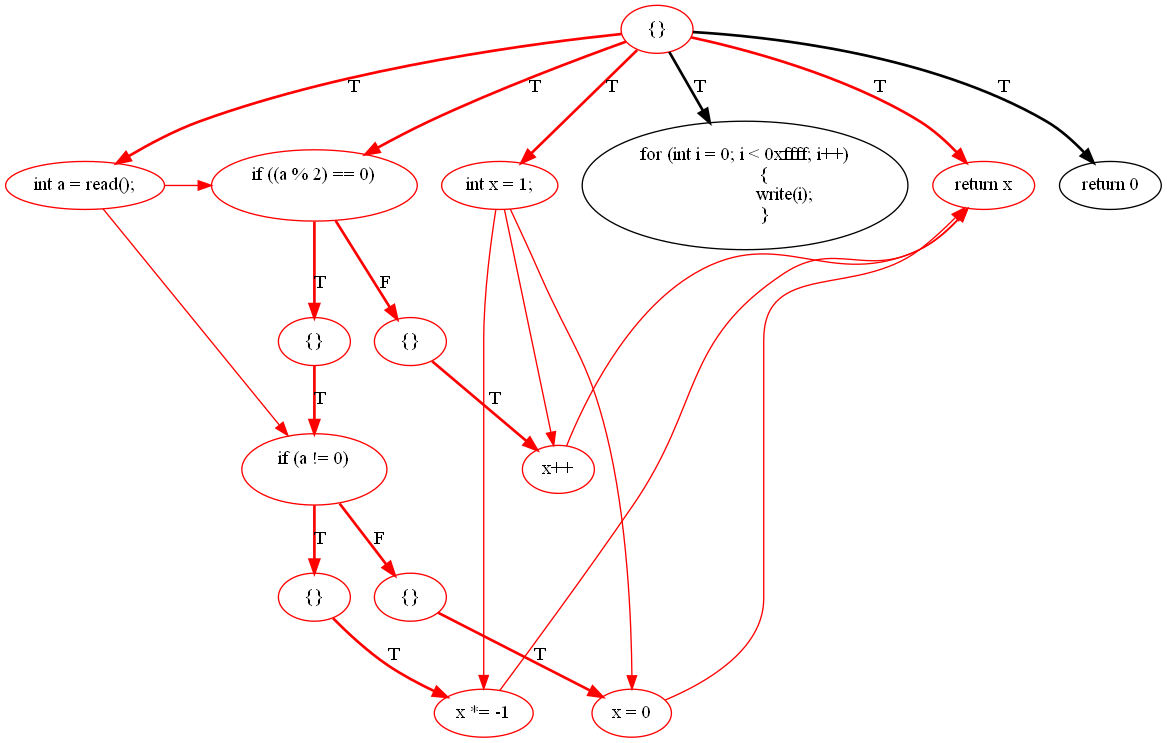
\includegraphics[scale=0.35]{pdg_sliced}
\caption{Sliced PDG. This figure showcases 
the PDG of the listing~\ref{lst:simpleexample}.
Red edges indicate the sliced part of the program w.r.t.
$C = (write(x)_{42}, \{x\})$.}
\label{img:pdg}
\end{figure}

Figure~\ref{img:pdg} shows a PDG that was extracted using an AST Slicer.
Nodes of the graph contain the same statements as seen in the code.
Frameworks that achieve such mapping between the code and the internal
control and data flows allow developers to create slicing tools much 
more easily.
One such framework is the LLVM/Clang Tooling library, which will be
talked about later.
The tool is available at \url{https://github.com/dwat3r/slicer}.

However, one can find many potential issues and obstacles when performing 
data flow analysis. 
Omitting the interprocedural slicing, as it is not relevant in this paper's
context, one is left with pointers and unstructured control flow.
While the latter is rarely used in single-threaded modern programming, 
the same cannot be said about the former. 

Pointers require us to extend the syntactic data flow analysis 
into a pointer or points-to analysis, which should be performed first. 
It is necessary to keep track of where pointers may point to (or must point to,
in case their address is not reassigned) during the execution. 
From this knowledge, other data flow edges must be created or
changed to accommodate the fact when the outgoing vertex mayhap writes
into a memory location possibly used by the incoming vertex. 

The analogical approach is then used for control dependency analysis since 
pointers might alter control flow as well. 
This change to control flow happens, namely when functions are called using 
function pointers.

The main advantage of static slicing is that it does not require
any runtime information. 
As program execution can be expensive both time-wise and resource-wise, 
static slicing offers program comprehension at a low cost. 
Because static slicing discovers program statements that can affect 
certain variables, it can remove dead code and be used for program segmentation. 

Furthermore, static slicing is used for testing software quality, maintenance, 
and test, all of which are relevant to this project.

\section{Dynamic slicing}

While the idea of building a program slice prevails, dynamic slicing 
drastically differs from static slicing in terms of input and the way
it is processed. 

\citet{Korel88} described a slicing approach that took into 
consideration information regarding a program's concrete execution. 
As opposed to static slicing, which builds a slice for any execution, 
dynamic slicing builds a slice for a given execution of a program. 
Using information available during a run of the program 
results in a typically much smaller slice.

\begin{lstlisting}[caption=Dynamic slice of the simple
  branching program, language=C++, label={lst:dynamicslice}]
#include<iostream>

void write(int x)
{
	std::cout << x << "\n";
}

int read()
{
	int x;
	std::cin >> x;
	
	return x;
}

int main(void)
{
	int x = 1;
	int a = read();
		
	x = 0;

	write(x);

	return 0;
}  
\end{lstlisting}

This decrease in size is mainly due to removing unnecessary 
branching of control statements and unexecuted statements in general. 
The slicing criterion now contains a set of the program's 
arguments in addition to the previous information. 
The location of the criterion's statement is also specified to avoid 
vagueness in the execution history. 

The criterion is therefore defined as follows.

\begin{defn}[Dynamic slicing criterion]\label{def02:6}
  Let $\mathcal{H} = (s_{x1},\dots,s_{xn})$ be an execution history of a program 
  $\mathcal{P} = (\{s_1,\dots,s_m\}, V)$, where $s_i$ denotes a statement
  and V is a set of variables $v_1,\dots,v_k$.
  Any triple $C = (h_i, V', \{a_1,\dots,a_j\})$, such that $h_i \in \mathcal{H}$,
  $V' \subseteq V$, $\forall v_i \in V': v_i$ is present in $h_i$,
  and $\{a_1,\dots,a_j\}$ is the input of the program,
  is called a \emph{slicing criterion}.
\end{defn}

The example listing~\ref{lst:dynamicslice} was computed from the original
listing~\ref{lst:simpleexample}. 
The criterion was set to $C = (write(x)_{42}, \{x\}, \{2\})$.
Since the dynamic slicer witnessed the program's execution,
it could precisely reduce the code to only those statements
that were executed. The result is a significantly smaller slice
than in the case of~\ref{lst:staticslice}.
Note that branching statements are gone.

Since dynamic slicing requires the user to run the program, 
it is typically used in cases where the execution with a fixed 
input happens regardless. Such cases include debugging and testing. 
For debugging, dynamic slices must reflect the subsequent restriction: 
a program and its slices must follow the same execution paths.

\section{Summary}

While the described program minimizing and debugging approaches have been 
formulated more than two decades ago, there have not been nearly enough 
successful attempts at implementing them. 

With each approach having its clear positives and negatives, 
it would be interesting to see how they handle program minimization. 
When cleverly used, a combination of these methods might 
result in a reasonably fast and inexpensive algorithm 
for the reduction of program size.
